\documentclass[a4paper,12pt]{article}
\usepackage{polytechnique}
\usepackage[french]{babel}
\usepackage{fontspec}
\usepackage{graphicx}
\usepackage{amsmath}
\usepackage{amssymb}
\usepackage{listings}
\usepackage{color}
\usepackage{hyperref}
\newcommand{\dps}{\displaystyle}
\renewcommand{\C}{\mathbb{C}}
\newcommand{\Q}{\mathbb{Q}}
\newcommand{\I}{\mathbb{I}}
\newcommand{\R}{\mathbb{R}}
\newcommand{\Z}{\mathbb{Z}}
\newcommand{\K}{\mathbb{K}}
\newcommand{\N}{\mathbb{N}}
\newcommand{\M}{\mathbb{M}}
\newcommand{\Lim}{\displaystyle\lim}
\newcommand{\ol}{\overline}
\renewcommand{\Pr}{\mathbb{P}}
\newcommand{\cffig}[1]{(\textit{Figure} \ref{#1})}

\begin{document}
\title{Rapport inf443}
\author{Brugere Tristan}
\maketitle
\tableofcontents{}

\lstset{language=C++,
                basicstyle=\ttfamily,
                keywordstyle=\color{blue}\ttfamily,
                stringstyle=\color{red}\ttfamily,
                commentstyle=\color{gray}\ttfamily,
                morecomment=[l][\color{magenta}]{\#}
}

\section{Introduction}
Le but du projet était de faire un jeu simple où un pigeon volant en ligne droite devrait éviter des immeubles.
Le plus simple pour comprendre le gameplay est soit de lancer l’éxécutable pgm, soit de regarder la vidéo « smaller.mp4 » montrant le gameplay.

\subsection{compilation}
Pour compiler le jeu, il suffit de se placer dans un répertoire où l’on veut construire l’éxecutable, disons build/
et de taper les commandes : 
\begin{lstlisting}[language=bash]
$ cmake .. # créer le makefile
$ make # compiler le projet
\end{lstlisting}

Après cela, on peut lancer le programme avec la commande

\begin{lstlisting}[language=bash]
$ ./pgm
\end{lstlisting}

\section{Spécificités du code et techniques mises en œuvre}

\begin{figure}[h]
  \centering
    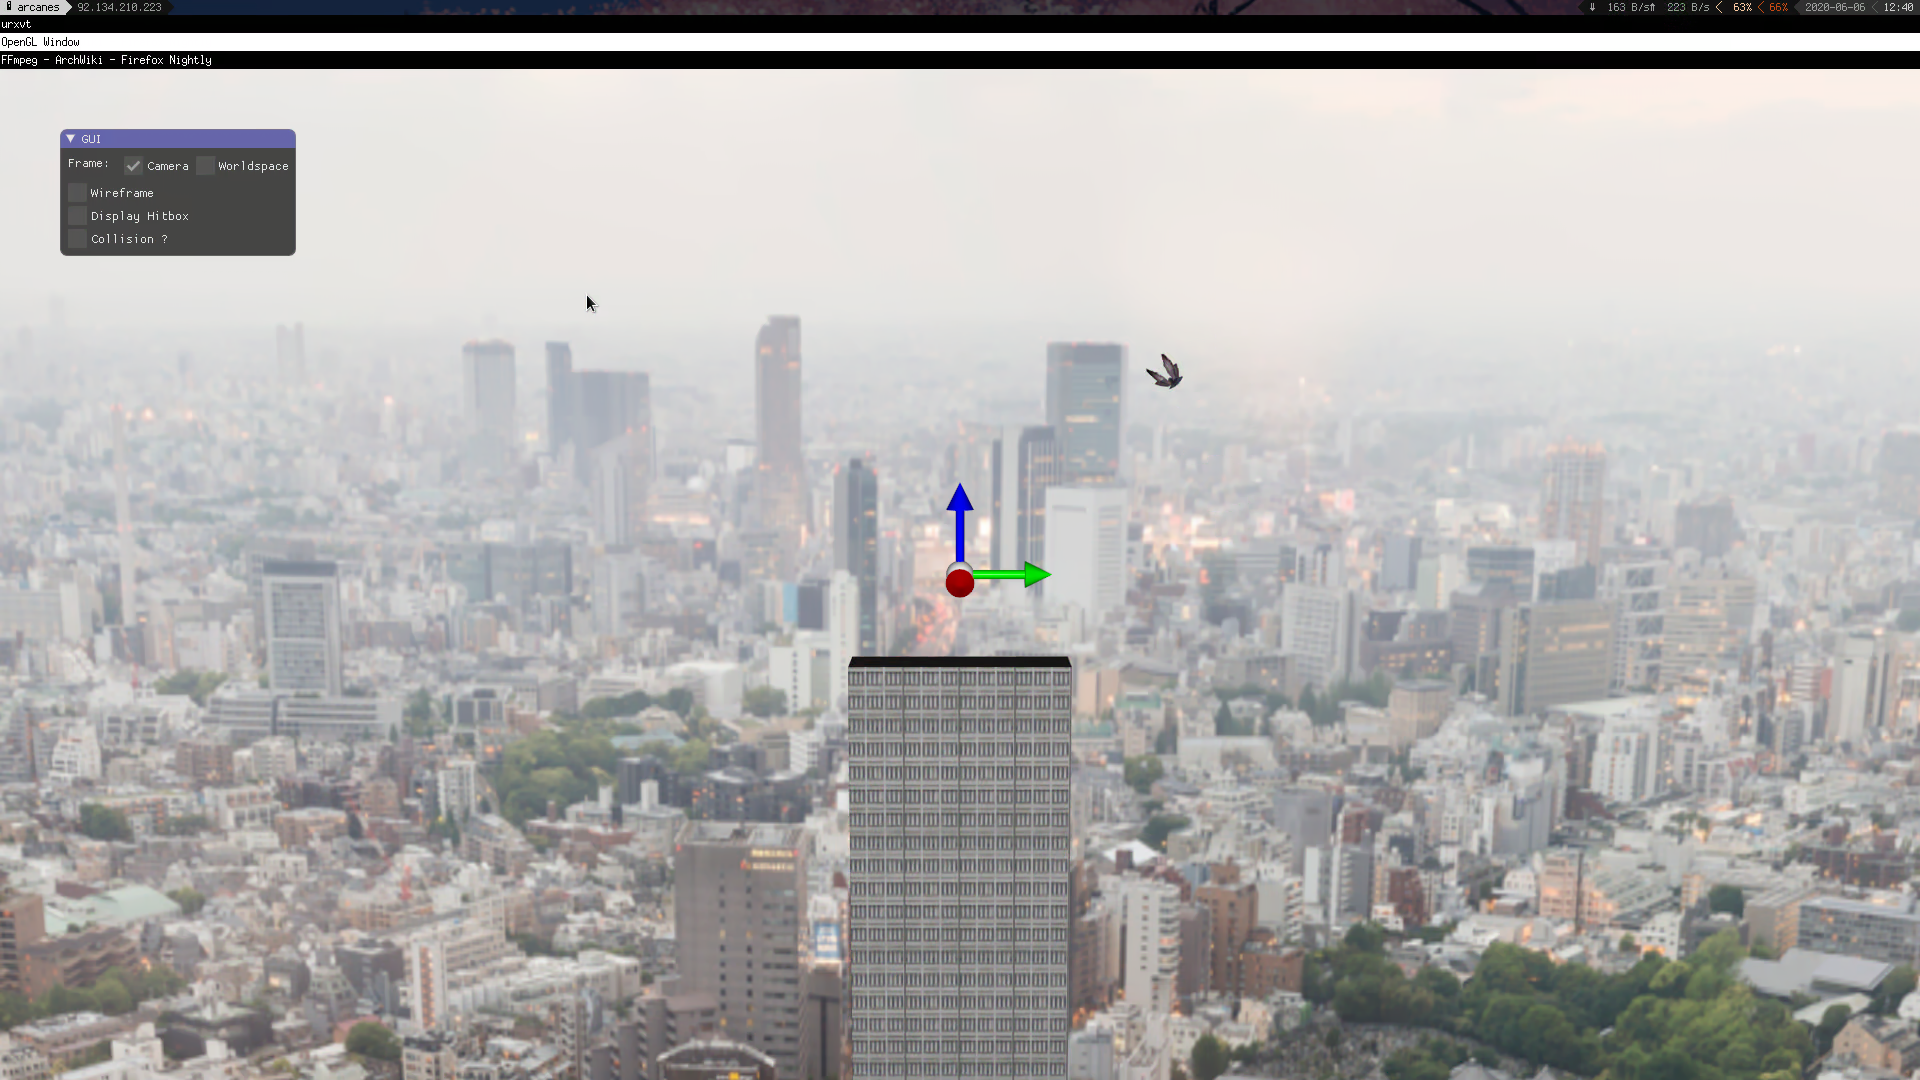
\includegraphics[width=\textwidth]{screenshot.png}
  \caption{une capture d’écran du gameplay}~\label{fig:bars1}
\end{figure}

\subsection{Organisation du code}

Le code de la scène se situe dans \verb|scenes/3D_graphics/00_default/|. Les ressources (textures, meshes) se situent dans le dossier resources/. 
À noter qu’il ne suffit pas pour que le projet fonctionne de copier ces dossiers, car le projet comprend aussi une petite modification dans la librairie vcl (dans la composition des transformations affines).

Le dossier \verb|00_default| contient 3 paires de fichiers.
\begin{itemize}
    \item \verb|default.[ch]pp| contient le code général de la scène
        (meshes hors personnage, mouvement de ces meshes…). 
    \item \verb|Character.[ch]pp| contient le code permettant de 
        charger, texturer, animer, et gérer la physique du personnage (l’oiseau).
    \item \verb|Hitbox.[ch]pp| contient le code de gestion des collisions.
\end{itemize}

\subsection{Textures et Uv mapping}
Une bonne partie du temps alloué au projet fut utilisée pour l’écriture des uv maps et le dessin des textures (même si cette partie n’est pas forcément visible dans le coffre).
Elles sont trouvables dans le dossier resources/textures du projet (ainsi que les maps uv des meshes).

Pour les textures de l’immeuble, je les ai téléchargées sur textures.com. Pour le pigeon, je les ai dessinées sur Gimp à partir de photos de pigeon ou de parties du corps de pigeon (détourées, redimensionnées, et améliorées au besoin). Le résultat n’est pas photoréaliste, et je n’ai par exemple pas dessiné l’avant de la tête qui n’est pas visible dans le jeu, mais il fait très bien illusion à la distance où se trouve la caméra (et ce même quand elle se trouve moins loin que dans la vidéo de démonstration. Pour déplacer la caméra, il suffit de modifier la variable \verb|camera_offset| dans le code).

% Parler de la "skybox"
Pour le décor, je n’ai pas utilisé une skybox à proprement parler : ce n’était pas nécessaire puisque la caméra ne tourne ni ne se déplace. Le décor est donc un simple panneau (style billboard) face à la caméra, à une distance notée horizon dans le code.
Pour que le décor rende correctement (\textit{ie.} pour éviter les effets de lumière étranges), j’ai simplement réglé ses paramètres à « specular = 0, diffuse = 0, ambiant = 1 ». 

\subsection{Gameplay et moteur physique}

La caméra se situe face à l’axe x, l’axe y vers la droite, et l’axe z vers le haut, comme on peut le voir sur la screenshot \cffig{fig:bars1}.


\textit{mouvement des immeubles :}

Pour simplifier le code, il est bon de comprendre que la caméra et l’oiseau ne se déplacent pas selon l’axe des x. Ce sont les obstacles (les immeubles) qui se déplacent vers la caméra (selon les x croissants).
Les immeubles ne se déplacent pas en ligne droite selon l’axe des x, ils se déplacent aussi selon l’axe des z (hauteur) pour simuler (un peu exagérément) la courbe de la terre. On a approximé localement la courbe de la terre à une fonction quadratique (Développement linéaire à l’ordre 2). 

Techniquement, les immeubles sont en fait tous le même mesh, qui est déplacé à toutes les positions des immeubles et redessiné à chaque fois (comme les arbres dans les TD). Ainsi les immeubles sont représentés par la structure \verb|building_positions|, qui est une file (structure FIFO).

On utilise un timer pour les générer périodiquement à une distance qu’on appelle « horizon ». Puisque les x des positions décroissent uniformément au cours du temps, les positions dans la structure \verb|building_positions| sont toujours décroissantes (les positions qui viennent d’être ajoutées sont les dernières dans la structure, et ont les x le plus petit (dans les négatifs)).

%garbage collect
Quand un immeuble dépasse la caméra (ie quand son x dépasse $offset\_camera + building\_size$), on le supprime. À noter que le fait que les x soient décroissants dans la structure des positions fait qu’il suffit de regarder les positions au début de la liste, jusqu’à ce qu’on n’ait plus besoin de supprimer, et non de parcourir toutes les positions (d’où la structure de file).
De même quand on testera les collisions avec l’oiseau, il sera seulement utile de tester les immeubles avec un x proche de 0, c’est-à-dire les premiers immeubles.

\textit{mouvement de l’oiseau :}

L’oiseau se déplace seulement dans le plan (y, z) orthogonal à la caméra (puisque c’est le reste du décor qui se déplace sur x).

Tout le code en rapport avec l’oiseau (son chargement, son animation et ses déplacements) est placé dans la classe \verb|Character| (dans Character.[ch]pp)

On a choisi les contrôles suivants : les flèches gauche et droite permettent de changer l’inclinaison de l’oiseau. La barre d’espace permet de donner un coup d’ailes qui applique sur l’oiseau une force vers le haut, selon son inclinaison (voir la vidéo ou tester le programme pour comprendre).
La physique de l’oiseau est simulée grâce à la méthode d’Euler, les forces s’appliquant étant la gravité, le cas échéant la force exercée par le mouvement d’ailes, ainsi qu’une force de frottement fluide.
Toutes les constantes liées à ces forces (et plus généralement à l’oiseau) sont dans la classe \verb|Character|.


\subsection{Gestions des collisions}

La gestion des collisions se situe dans la classe \verb|Hitbox|. On utilise des parallélépipèdes rectangles parallèles 
aux axes pour gérer les collisions.

Les hitbox des immeubles rectangulaires sont les immeubles eux-mêmes. 
Pour l’oiseau, on utilise une seule hitbox, mais on faut évoluer sa forme selon l’animation pour être le plus proche possible de la forme de l’oiseau 
(on le voit bien dans la vidéo, ou en cochant la case « display hitbox » dans le programme).

\subsection{Personnage et animations}

L’oiseau est représenté par la classe \verb|Character| qui hérite de la classe \verb|hierarchy_mesh_drawable|.
Chaque aile est représentée par deux meshes, la queue et le reste du corps sont deux meshes indépendants (pour un total de 6 meshes).

Elle possède en plus les fonctions de déplacement, et le code pour charger ses meshes, et gérer son animation.
Il suffit d’appeler sa méthode \verb|draw| pour que l’animation soit gérée automatiquement (selon si on est en train de donner un coup d’aile).

\section{Conclusion}

C’était un projet ludique (création d’un jeu), qui m’a permis de mettre en application de nombreux concepts vus en cours (simulation physique, animation, gestion des matériaux (diffus, specular, ambiant)) 
et dans les TD (textures et maps uv, animation).

Le jeu a encore quelques problèmes (le point de vue rend difficile l’appréciation des distances, il est possible de sortir du cadre, les constantes ne sont pas tout à fait optimisées…) mais est fonctionnel, 
et m’a permis d’en apprendre beaucoup sur la conception d’un jeu, ainsi que de renouer avec les outils de 
création graphique que je n’avais pas utilisés depuis longtemps (Blender et GIMP).

\subsection{Améliorations}
On pourrait apporter de nombreuses améliorations que je n’ai pas eu le temps d’inclure, dont en voici quelques-unes :
\begin{enumerate}
    \item Un meilleur cadrage de la caméra (une caméra plus en plongée permettrait une meilleure évaluation des distances)
    \item Une gestion des collisions plus avancées (on pourrait donner plusieurs hitbox au personnage, la classe \verb|Hitbox| permettrait de ce faire très facilement)
    \item Un système de score pour rendre le gameplay plus dynamique.
    \item Plus d’obstacles, et des bonus par lesquels il faudrait passer (pour rendre le gameplay plus intéressant)
\end{enumerate}


\end{document}

